\section{ПРОГРАМНА РЕАЛІЗАЦІЯ СИСТЕМИ ДЛЯ УПРАВЛІННЯ КОРИСТУВАЧАМИ, ДОКУМЕНТАМИ, ЗАВДАННЯМИ І МОЖЛИВОСТІ СПІЛЬНОЇ РОБОТИ}
\subsection{Реалізація роботи бази даних}
\par Загальна структура бази даних зображено на рисунку \ref{pic:db_shema}. Весь код для створення бази даних реалізовано мовою SQL, за допомогою запитів до БД.
\par Зовнішні посилання створено за допомогою команди <<reference>>. Для прикладу код для створення таблиці користувачів (worker), котра має чотири зовнішні ключі які посилаються на таблиці команди (team), роль користувача (role\_name), тип посади (job\_type\_name) та регіон (region\_name) користувачів. Відповідно таким чином і реалізовано всі решта таблиць:

\begin{lstlisting}[language=SQL]
DROP TABLE IF EXISTS `worker`;
/*!40101 SET @saved_cs_client     = @@character_set_client */;
/*!40101 SET character_set_client = utf8 */;
CREATE TABLE `worker` (
  `id` bigint(20) NOT NULL AUTO_INCREMENT,
  `birthday` date DEFAULT NULL,
  `date_hire` date DEFAULT NULL,
  `login` varchar(255) NOT NULL,
  `name` varchar(255) NOT NULL,
  `pass` varchar(255) NOT NULL,
  `phone` varchar(255) DEFAULT NULL,
  `photo` longblob,
  `private_mail` varchar(255) DEFAULT NULL,
  `street` varchar(255) DEFAULT NULL,
  `surname` varchar(255) NOT NULL,
  `version` int(11) DEFAULT NULL,
  `job_type_name` bigint(20) NOT NULL,
  `region_name` bigint(20) NOT NULL,
  `role_name` bigint(20) DEFAULT NULL,
  `team_name` bigint(20) NOT NULL,
  `mobile` varchar(255) DEFAULT NULL,
  PRIMARY KEY (`id`),
  UNIQUE KEY `login` (`login`),
  KEY `FKD162537E30271785` (`team_name`),
  KEY `FKD162537EB0DD720C` (`job_type_name`),
  KEY `FKD162537E520C2F83` (`role_name`),
  KEY `FKD162537EBDECCB25` (`region_name`),
  CONSTRAINT `FKD162537E30271785` FOREIGN KEY (`team_name`) REFERENCES `team` (`id`),
  CONSTRAINT `FKD162537E520C2F83` FOREIGN KEY (`role_name`) REFERENCES `worker_role` (`id`),
  CONSTRAINT `FKD162537EB0DD720C` FOREIGN KEY (`job_type_name`) REFERENCES `worker_job_type` (`id`),
  CONSTRAINT `FKD162537EBDECCB25` FOREIGN KEY (`region_name`) REFERENCES `region` (`id`)
) ENGINE=InnoDB AUTO_INCREMENT=3 DEFAULT CHARSET=utf8;
/*!40101 SET character_set_client = @saved_cs_client */;	
\end{lstlisting}
\par Посилання на інші таблиці на веб інтерфейсі реалізовано за допомогою випадаючих списків -- це дає можливість забезпечити введення вірних даних і допомагає відобразити вже існуючі в базі даних записи.
Для прикладу візьмемо форму для створення нового користувача та вибору регіону, що зображено на рисунку \ref{pic:page_drop_down}.


\begin{figure}[!ht]
\centering
    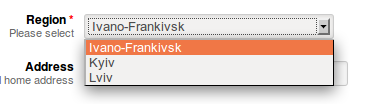
\includegraphics[width=0.5\textwidth]{page_drop_down.png}
    \vspace{18pt}
    \captionof{figure}{Вибір регіону при створенні користувача}\label{pic:page_drop_down}
\end{figure}


\subsection{Реалізація веб інтерфейсу}
\par Веб інтерфейс користувача повинний бути зручний та інтуїтивно зрозумілий кожному користувачеві, тому його було реалізовано в легких тонах та зручно розташовано всі навігаційні елементи.

\begin{figure}[!ht]
\centering
		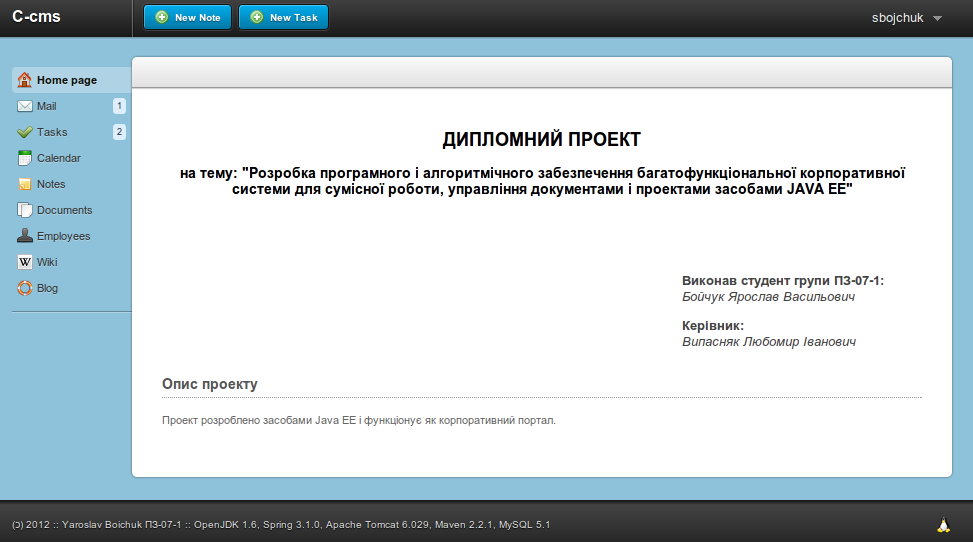
\includegraphics[width=1.00\textwidth]{page_main.png}
    \vspace{18pt}
		\captionof{figure}{Загальний інтерфейс програмного продукту}\label{pic:page_main}
\end{figure}
\par Весь інтерфейс сайту поділяється на три основні компоненти: головний блок, навігаційна панель, головне меню. Для зручності розробки цих компонентів використано Apache Tiles, що дає змогу поділяти код на логічні одиниці.
\begin{lstlisting}
<body>
 <div id="wrapper">
  <header>
   <tiles:insertAttribute name="header" ignore="true" />
  </header>
  <section>
   <div class="container_8 clearfix">
    <tiles:insertAttribute name="menu" ignore="true" />
    <tiles:insertAttribute name="body" />
   </div>
   <div id="push"><!-- --></div>
  </section>
 </div>
  <footer>
   <tiles:insertAttribute name="footer" ignore="true" />
  </footer>
 <div class="apple_overlay black" id="overlay">
  <a class="close"></a>
  <iframe class="contentWrap" style="width: 100%; height: 500px"></iframe>
 </div>
 <div style="display: none; position: absolute;" id="calroot">
  <div id="calhead">
   <a id="calprev"></a>
   <div id="caltitle"></div>
   <a id="calnext"></a>
  </div>
  <div id="calbody">
   <div id="caldays">
    <span>Sun</span><span>Mon</span><span>Tue</span><span>Wed</span><span>Thu</span><span>Fri</span><span>Sat</span>
   </div>
   <div id="calweeks">
    <!--   -->
   </div>
  </div>
 </div>
</body>
\end{lstlisting}



\subsubsection{Навігаційна панель}
\par На навігаційній панелі розташовані елементи швидкого доступу до завдань та задач.
З легкістю можна додати будь-яке завдання, при чому вибрати заголовок завдання, детальний опис та кінцевий час виконання (рисунок \ref{pic:page_navigation_new_task});

\par Для зручності навігаційна панель рухається разом із прокруткою сторінки, тобто якщо навіть користувач перейде в низ сторінки, то йому панель буде завжди доступна -- це зроблено для простоти і швидкості доступу до створення нової нотатки та завдання.
\par Справа на навігаційній панелі розташовано меню користувача. Тут знаходиться кнопка переходу на профіль робочого та кнопка виходу із сайту (рисунок \ref{pic:page_navigation_profile}). Після виходу всі дані, які збережені в сесії будуть видалені.

\begin{figure}[!ht]
\centering
    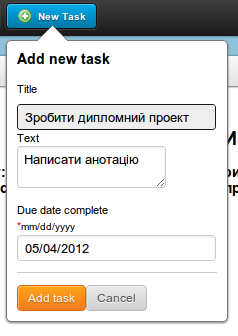
\includegraphics[width=0.3\textwidth]{page_navigation_new_task.png}
    \vspace{18pt}
    \captionof{figure}{Приклад створення завдання із навігаційної панелі}\label{pic:page_navigation_new_task}
\end{figure}

\begin{figure}[!ht]
\centering
    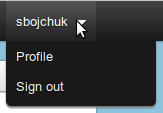
\includegraphics[width=0.3\textwidth]{page_navigation_profile.png}
    \vspace{18pt}
    \captionof{figure}{Панель користувача}\label{pic:page_navigation_profile}
\end{figure}


\subsubsection{Головне меню}
\par Навігація по веб ресурсу реалізована за допомогою головного меню. В головному меню відображаються всі доступні на сайті навігаційні посилання:
\begin{itemize}
  \item головна сторінка;
  \item корпоративна пошта;
  \item завдання;
  \item календар;
  \item нотатки;
  \item документи;
  \item список робочих;
  \item корпоративна вікі;
  \item блог.
\end{itemize}
\par При переході на будь-яке меню, воно зразу підсвічується -- це зроблено для зручності користувачеві, щоб було зразу видно де він знаходиться в даний момент часу. Програмно це відбувається за допомогою передачі з контролера в модель атрибута із назвою меню:
\begin{lstlisting}[language=Java]
uiModel.addAttribute("menu", "NOTE");
\end{lstlisting}
\par Потім в JSP вигляді головного меню відбувається перевірка на значення поточного меню, і якщо воно сходиться із атрибутом <<menu>> то додається css клас <<active>> (рисунок \ref{pic:page_menu}):

\begin{lstlisting}
<c:choose>
<c:when test="${menu eq 'NOTE' }"><li class="active"><a class="nav-icon icon-note" href="/ccms/notes">Notes</a></li></c:when>
<c:otherwise><li><a class="nav-icon icon-note" href="/ccms/notes">Notes</a></li></c:otherwise>
</c:choose>
\end{lstlisting}

\par Відповідно до переходу на певний пункт, відбувається запит контролеру MVC, і вибірка даних із бази даних через контролер з подальшою передачею на вигляд. Для прикладу запит для запису в базу даних та перевірка на валідність даних:
\begin{lstlisting}
@RequestMapping(method = RequestMethod.POST, produces = "text/html")
public String create(@Valid Note note, BindingResult bindingResult, Model uiModel, HttpServletRequest httpServletRequest) {
    if (bindingResult.hasErrors()) {
        populateEditForm(uiModel, note);
        uiModel.addAttribute("menu", "NOTE");
        return "redirect:/notes";
    }
    uiModel.asMap().clear();
    note.setAuthor(Worker.getPrincipal());
    note.setDatetime(new Date());
    note.persist();
    uiModel.addAttribute("menu", "NOTE");
    return "redirect:/notes";
}
\end{lstlisting}

\begin{figure}[!ht]
\centering
    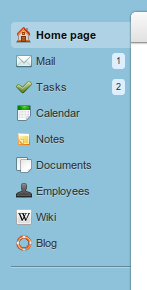
\includegraphics[width=0.30\textwidth]{page_menu.png}
    \vspace{14pt}
    \captionof{figure}{Навігаційне меню порталу}\label{pic:page_menu}
\end{figure}


\subsection{Робота із даними}
\par Для маппінгу даних із форми до бази даних використовується JPA із Hibernate фреймворком поверх нього. Для кожної форми створюється певний домен (по своїй суті persistence bean), котрий за допомогою анотацій із пакету Javax дає змогу переносити об'єкти Java в базу даних (за допомогою використання мови запитів Hibernate Query Language). Для прикладу bean для запису нотаток в базу даних:
\begin{lstlisting} 
@Configurable
@Entity
public class Note {

@NotNull
private String title;

@NotNull
@Size(max = 1000000)
private String text;

@Temporal(TemporalType.TIMESTAMP)
@DateTimeFormat(style = "M-")
private Date datetime;

@ManyToOne
private Worker author;

public static TypedQuery<Note> findNotesByAuthorEquals(Worker author) {
    if (author == null)
        throw new IllegalArgumentException("The author argument is required");
    EntityManager em = Note.entityManager();
    TypedQuery<Note> q = em.createQuery("SELECT o FROM Note AS o WHERE o.author = :author ORDER by o.id DESC", Note.class);
    q.setParameter("author", author);
    return q;
}

public String getTitle() {
    return this.title;
}

public void setTitle(String title) {
    this.title = title;
}
\end{lstlisting}
\par В вище наведеному коді кожне поле має свій метод на getter та setter, що дає змогу вибірки даних, та статичний метод <<findNotesByAuthorEquals>> для пошуку повідомлень даного автора, що дає змогу в любому місці здійснити операції щодо пошуку цих повідомлень.

\subsection{Категорії порталу}
\subsubsection{Авторизація користувачів на веб-порталі}
\par Сторінка авторизації пропонує користувачеві ввести свій логін та пароль (рисунок \ref{pic:page_login}) та у випадку неправильних даних буде відображена помилка (рисунок \ref{pic:page_login_error})

\begin{figure}[!ht]
\centering
    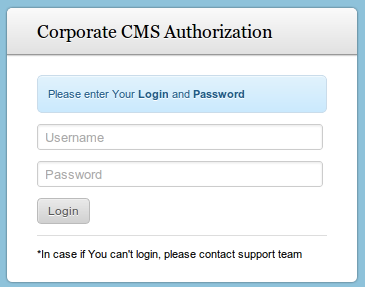
\includegraphics[width=0.50\textwidth]{page_login.png}
    \vspace{18pt}
    \captionof{figure}{Форма авторизації користувача}\label{pic:page_login}
\end{figure}

\begin{figure}[!ht]
\centering
    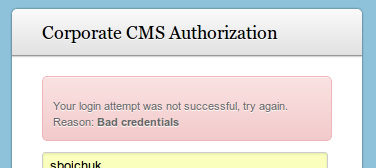
\includegraphics[width=0.50\textwidth]{page_login_error.png}
    \vspace{18pt}
    \captionof{figure}{Помилка авторизації користувача}\label{pic:page_login_error}
\end{figure}

\par Якщо введено вірні дані, то відбувається запис нової сесії в пам'ять та перенаправлення користувача на головну сторінку, або на сторінку із якої прийшов користувач.

\subsubsection{Корпоративна пошта}
\par Всі отримані листи користувач може переглянути в пункті пошта. Напроти меню <<пошта>> відображається кількість не прочитаних повідомлень (рисунок \ref{pic:page_mail}).
  \begin{figure}[!ht]
  \centering
      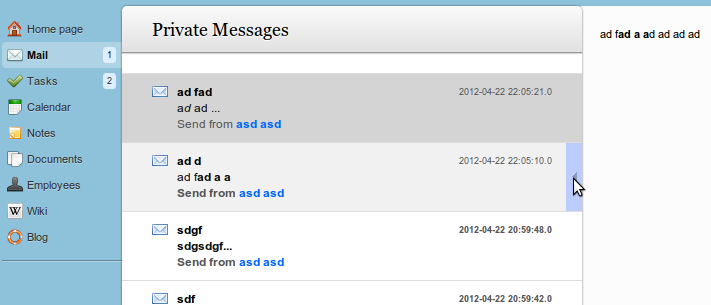
\includegraphics[width=1\textwidth]{page_mail.png}
      \vspace{18pt}
      \captionof{figure}{Сторінка зі списком повідомлень}\label{pic:page_mail}
  \end{figure}
\par Над кожним повідомленням показано тему повідомлення. Головний текст повідомлення обрізаний, проте коли клікнути на повідомлення, збоку висунеться панель із повним описом повідомлення. Також під повідомленням показано час відправлення повідомлення та відправник повідомлення. При кліку на відправника, відбудеться перехід на його персональну сторінку. Кожне не прочитане повідомлення виділяється сирім кольором, для того щоб легше було його знайти, і при детальному перегляді його, колір забереться, і кількість повідомлень, що показуються біля меню -- буде зменшено.
\par Відправлення повідомлення можливе із персональної сторінки кожного користувача. Після переходу на персональну сторінку, слід надрукувати тему повідомлення та саме повідомлення (рисунок \ref{pic:page_send_message}).
  \begin{figure}[!ht]
  \centering
      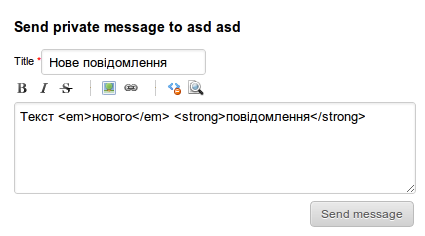
\includegraphics[width=0.8\textwidth]{page_send_message.png}
      \vspace{18pt}
      \captionof{figure}{Форма для відправлення повідомлень}\label{pic:page_send_message}
  \end{figure}
\par Зразу також доступний WYSIWYG редактор і онлайн перегляд повідомлення яке друкується. Доставка повідомлення відбувається моментально, адже використовується локальний сервер бази даних.

\subsubsection{Персональний календар для збереження подій}
Персональний календар дає змогу показати всі занесені до нього нотатки та записи. Перегляд даних можливий у трьох проміжних режимах: на місяць, на тиждень (рисунок \ref{pic:page_calendar}) та на день.
  \begin{figure}[!ht]
  \centering
      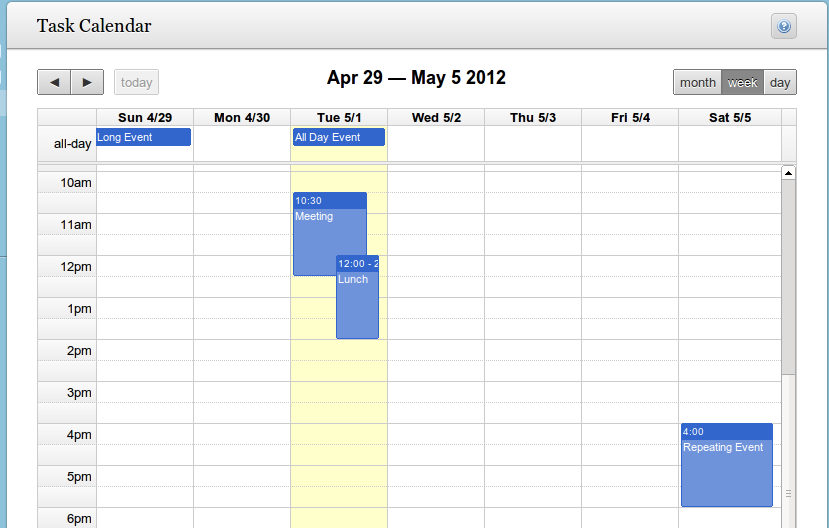
\includegraphics[width=1\textwidth]{page_calendar.png}
      \vspace{18pt}
      \captionof{figure}{Завдання на тиждень}\label{pic:page_calendar}
  \end{figure}
\par Завдання можуть бути додані як на певний проміжний період, так і на цілий день. Для маніпуляції записів в календарі використана технологія drag \& drop від jQuery.

\subsubsection{Завдання і задачі}
\par Категорія задач створена для збереження своїх задач (рисунок \ref{pic:page_navigation_new_task}) і можливістю їх перегляду в майбутньому. Це дає змогу всі свої важливі завдання тримати в одному місці (рисунок \ref{pic:page_task}).
  \begin{figure}[!ht]
  \centering
      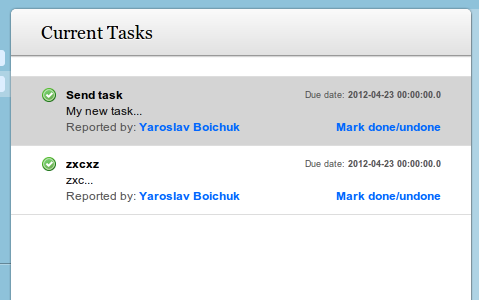
\includegraphics[width=0.7\textwidth]{page_task.png}
      \captionof{figure}{Поточні завдання}\label{pic:page_task}
  \end{figure}
\par Кожне завдання яке не виконано ще, позначається аналогічно до непрочитаного повідомлення -- сірим кольором, це дає змогу зразу побачити всі поточні завдання. 
\par Біля кожного завдання вказано хто створив дане завдання та кінцевий час його виконання. Також в головному меню навпроти пункту <<завдання>> вказується кількість невиконаних на даний момент завдань. Також кожне завдання може бути позначене як виконане або ж невиконане.

\subsubsection{Основні функції управління користувачами порталу}
\par Список всіх користувачів відображається в таблиці із деяким набором полів. Для переглядаючого доступні певні маніпуляції зі списком, такі як сортування та посторінкова навігація (рисунок \ref{pic:page_workers}). А у випадку, якщо користувач наділений правами адміністратора -- то має право на створення нового користувача (рисунок \ref{pic:page_create_worker}).

  \begin{figure}[!ht]
  \centering
      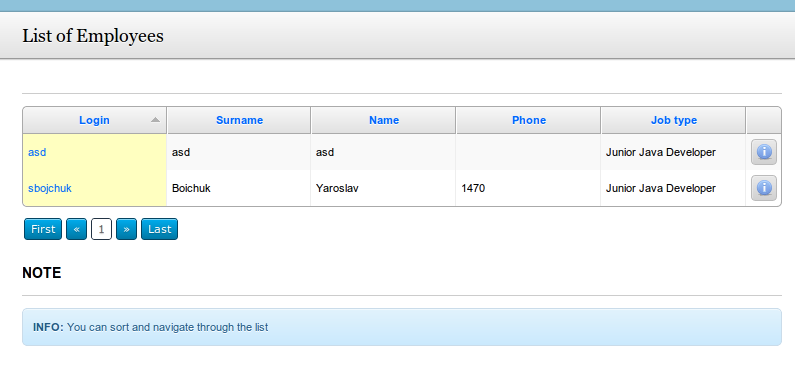
\includegraphics[width=1\textwidth]{page_workers.png}
      \par \
      \captionof{figure}{Список користувачів із можливістю сортування}\label{pic:page_workers}
  \end{figure}


\par Після переходу на сторінку користувача, у його профайлі буде відображена вся детальна інформація (рисунок \ref{pic:page_worker})
  
\par Якщо при введенні не валідних даних, або ж залишити незаповненим обов'язкове поле -- то буде повідомлена відповідна помилка, і дані не потраплять на перевірку на сервер. Якщо ж зловмиснику вдасться все ж таки обійти перевірку форми, то сам сервер не пустить додати не валідні дані до бази даних, оскільки всі дані перевіряються другий раз за допомогою binding result об'єкта та анотації @Valid:
\begin{lstlisting}
public String update(@Valid Worker worker, BindingResult bindingResult, Model uiModel, HttpServletRequest httpServletRequest) {

if (bindingResult.hasErrors()) {
    populateEditForm(uiModel, worker);
    uiModel.addAttribute("menu", "WORKER");
    return "workers/update";
}
\end{lstlisting}

\begin{center}
      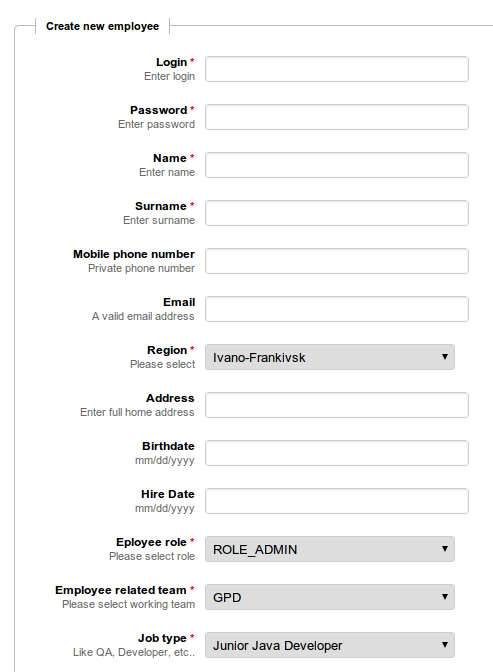
\includegraphics[width=0.7\textwidth]{page_create_worker.png}
      \par \
      \captionof{figure}{Створення нового користувача}\label{pic:page_create_worker}
  \end{center}

\par Якщо після проходження валідації є допущені помилки то дані назад <<повертаються>> на форму і відображається помилка. В іншому випадку, дані передадуться на модель та відбудеться запис у базу даних
\begin{lstlisting}
uiModel.asMap().clear();
worker.merge();
\end{lstlisting}


\subsubsection{Зберігання документів для спільного використання}
Дана категорія призначена для зберігання документів для їх спільного використання, для прикладу це можуть бути презентації, облікові документи чи просто інші нотатки. Для додавання доступні три категорії: презентації, текстові документи та таблиці. При завантаженні нового документа на портал, слід вказати категорію в котру повинен попасти документ, та вказати чи документ призначений для загально використання чи тільки для персонального.
\par Всі загальні документи доступні для завантаження та можливістю подальшого перегляду.

\begin{figure}[!ht]
  \centering
      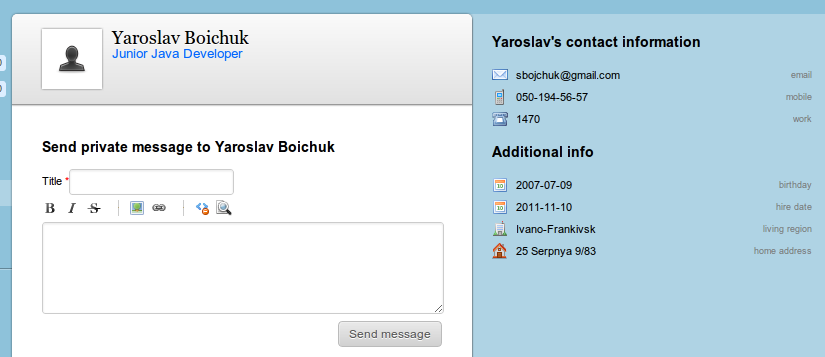
\includegraphics[width=1\textwidth]{page_worker.png}
      \par \
      \captionof{figure}{Профайл користувача}\label{pic:page_worker}
  \end{figure}

\subsubsection{Корпоративна wiki}
\par Корпоративна wiki в основному призначена для розповсюдження цікавої інформації між користувачами та являє собою єдине центральне сховище з можливість будь-якої маніпуляції документами. Кожна стаття має свою певну категорію -- що спрощує подальшу навігацію та пошук.

\subsubsection{Корпоративний блог}
\par Корпоративний блог має спільні риси із wiki, проте додати інформацію в нього тільки має право адміністратор та наділені такими правами групи користувачів. Основна ціль блогу -- це швидше інформування робочих про новини порталу та компанії.
